\chapter{Fundamentação Teórica}\label{chp:rev}



\begin{center}
    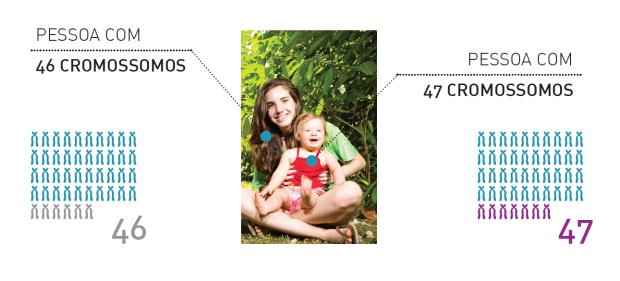
\includegraphics[width=1\linewidth]{figuras/sindrome de down.png}
    \captionof{figure}{Imagem comparativa de cromossomos entre pessoas com síndrome de down e pessoa sem a condição genética.}
    \label{fig:Cromossomos Comparativo pessoa normal e com sindrome de down}
    Fonte para a imagem\footnote{\url{https://emsinapse.wordpress.com/2017/10/12/post-especial-pe-dia-das-criancas-a-equoterapia-no-desenvolvimento-de-habilidades-em-criancas-com-a-sindrome-de-down/}}
\end{center}


A Síndrome de Down é uma condição genética causada pela presença de todo ou parte de uma cópia extra do cromossomo 21, o que resulta em deficiência intelectual e atrasos no desenvolvimento físico, cognitivo e motor. De acordo com \cite{schwartzman2003sindrome}, "É uma alteração genética, de causa desconhecida, ocorrida na divisão celular, logo após a concepção. Como consequência dessa alteração cromossômica, anomalias no desenvolvimento se manifestam já na vida intra-uterina, embora se tornem mais evidentes após o nascimento."

Essa síndrome possui características marcantes que possibilitam seu diagnóstico logo após o nascimento da criança. Dentre as características físicas mais comuns associadas à síndrome de Down estão olhos levemente oblíquos, nariz pequeno, pescoço mais curto, baixa estatura, mãos e pés pequenos, hiperflexibilidade, além de atrasos motores e intelectuais. "As pessoas com SD apresentam algumas características físicas bem definidas, como olhos amendoados, pregas palmares transversas únicas, língua protusa, braquicefalia, entre outras." \cite{coelho2016sindrome}.

Essa cópia extra do cromossomo afeta o desenvolvimento e está associada a características físicas e cognitivas distintas. Pode resultar em atrasos no desenvolvimento físico e intelectual, além de aumentar o risco de certas condições de saúde, como problemas cardíacos, visuais e dificuldades de aprendizado.

A trissomia do cromossomo 21 é causada por um erro na divisão celular, onde o cromossomo extra não é separado corretamente durante a formação dos óvulos ou espermatozoides. Quando ocorre a fecundação, essa célula com três cópias do cromossomo 21 se incorpora ao embrião.

Em termos mais técnicos, a trissomia 21 resulta em alterações genéticas que podem afetar a expressão dos genes importantes para um desenvolvimento normal. A presença desse cromossomo extra pode interferir na regulação genética, causando mudanças nas vias de sinalização celular e no funcionamento dos órgãos e sistemas corporais.

É fundamental destacar que cada pessoa com síndrome de Down pode manifestar características e dificuldades singulares, pois a manifestação e intensidade dos sintomas podem variar consideravelmente. É crucial contar com acompanhamento médico especializado e um plano de cuidado adequado para assegurar o melhor desenvolvimento e qualidade de vida para os indivíduos com síndrome de Down.

As pessoas com Síndrome de Down podem apresentar desafios intelectuais e motores. No entanto, quando estimuladas adequadamente desde a infância, podem aprender, desenvolver habilidades e alcançar uma vida produtiva e independente. Cabe à família, escola e sociedade apoiá-las para que alcancem seu máximo potencial. Desafios e ferramentas que auxiliam o aprendizado têm ajudado a superar essas dificuldades enfrentadas. O uso de tecnologias e mecanismos de aprendizado pode estimular e facilitar a interpretação e entendimento do conteúdo abordado em sala de aula, sendo uma extensão complementar para suprir necessidades de aprendizado e assimilação de uma forma mais lúdica e divertida para a criança.

As crianças com Síndrome de Down enfrentam desafios no aprendizado da matemática devido a dificuldades cognitivas relacionadas à condição. Problemas com contagem, reconhecimento de números, cálculos simples, raciocínio lógico e compreensão conceitual são comuns. A memória operacional limitada, lentidão no processamento de informações e déficits na habilidade de resolver problemas matemáticos dificultam o progresso. Para superar essas barreiras, o ensino deve ser multissensorial, com materiais concretos e atividades funcionais significativas, partindo do nível de desenvolvimento real da criança.

Apesar das limitações intelectuais e físicas, quando estimuladas e apoiadas de forma adequada desde a infância, as pessoas com Síndrome de Down são capazes de aprender, desenvolver habilidades sociais e conseguir uma vida adulta produtiva e independente. Cabe à família, escola e sociedade oferecer as condições necessárias para que essas pessoas alcancem seu máximo potencial.

\section{Desenvolvimento cognitivo}

As crianças com Síndrome de Down apresentam atraso no desenvolvimento cognitivo devido às alterações genéticas causadas pela trissomia do cromossomo 21. No entanto, o grau de comprometimento intelectual é bastante variável. De modo geral, elas costumam atingir os marcos do desenvolvimento motor e cognitivo mais tardiamente do que outras crianças. Por exemplo, o sentar, engatinhar e andar ocorrem por volta dos 2 aos 5 anos de idade. 

Já a linguagem tem início por volta dos 2 anos, com evolução mais lenta. Habilidades como vestir-se, alimentar-se e higiene pessoal também demandam mais tempo para serem dominadas. O quociente de inteligência das crianças com Down situa-se na faixa leve a moderada de deficiência intelectual. Mas com estímulos adequados e intervenção precoce, elas podem maximizar seu potencial cognitivo.

Cada criança irá apresentar um ritmo diferente de aprendizagem. É papel dos pais e educadores identificar suas necessidades individuais e trabalhar habilidades como comunicação, raciocínio, memória, atenção e socialização. Fornecer um ambiente enriquecido, com atividades lúdicas e pedagógicas guiadas, ajuda no desenvolvimento cognitivo das crianças.

\section{Atraso na fala e Linguagem}

O atraso no desenvolvimento da fala e linguagem é muito comum em crianças com Síndrome de Down. A maioria apresenta algum nível de comprometimento na comunicação verbal.Isso ocorre por diversos fatores relacionados à condição, como hipotonia muscular, alterações anatômicas na boca e garganta, déficit cognitivo e atraso no desenvolvimento motor. Todos esses aspectos dificultam a aquisição e o uso da linguagem falada.

As crianças com Down frequentemente começam a falar mais tarde do que o esperado, entre os 2 e 3 anos. Além disso, a progressão da fala tende a ser mais lenta. Elas podem ter dificuldade para pronunciar certos sons da língua, limitando o vocabulário.A compreensão da linguagem oral também pode estar prejudicada. Isso amplia os desafios de comunicação, pois a criança não entende tudo o que lhe é dito.Para auxiliar no desenvolvimento da fala, é importante que pais e professores estimulem a comunicação desde cedo. Fazer terapia fonoaudiológica e usar outros recursos aumentativos, como imagens e gestos, também é essencial.Com paciência, dedicação e os estímulos adequados, as crianças com Down syndrome podem desenvolver boas habilidades de comunicação verbal. Mas é preciso entender suas limitações e buscar formas de facilitar a interação.

\section{Desafios Sociais e comportamentais}


As crianças com Síndrome de Down podem apresentar vários desafios comportamentais que requerem atenção e apoio especiais dos pais, cuidadores e educadores. Algumas das dificuldades mais comuns incluem problemas de comunicação, hiperatividade e desafios sensoriais. Muitas crianças com Down têm atrasos no desenvolvimento da fala e linguagem, o que pode gerar frustração e problemas de comportamento. É importante oferecer a elas métodos alternativos de comunicação e ser paciente para entender suas necessidades. Além disso, algumas podem exibir sintomas de TDAH, com dificuldades de concentração e impulsividade. 

Outro desafio comum são as sensibilidades sensoriais. As crianças com Down podem ser hipersensíveis ou hipossensíveis a certos estímulos, levando a comportamentos como busca sensorial ou evitação. As rotinas e transições também podem ser difíceis para elas. Oferecer um ambiente estruturado e expectativas claras ajuda a mitigar esses problemas. Além disso, assim como qualquer criança, aquelas com Down podem apresentar teimosia e comportamentos de oposição. É importante estabelecer limites claros e usar estratégias de reforço positivo para incentivar um comportamento adequado.

 Buscar orientação de profissionais da saúde, terapeutas e grupos de apoio especializados em Síndrome de Down pode fornecer insights e recursos valiosos para lidar com os desafios comportamentais dessas crianças. Cada uma é única, e o que funciona para uma pode não funcionar para outra. Personalizar intervenções e estratégias para atender às necessidades e pontos fortes específicos da criança é essencial.

\section{Ensino de Matemática Básica para Crianças com Síndrome de Down }

Segundo \cite{fonseca2016concepccao}, a educação escolar por muitos anos foi apenas direito de poucos, mas com o passar das décadas tornou-se direito de todos. Na atualidade se busca assegurar que este direito seja garantido a toda a população e que sejam atendidas as demandas dos ditos diferentes no processo de aprendizagem. Para tanto a educação de pessoas com deficiência visando melhorias, passou por várias reformulações e modificações nas legislações. Sobretudo com as lutas de pessoas com deficiência e de seus familiares, em função disso temos hoje amparo na legislação no que se refere à educação das pessoas com deficiência 

A política de inclusão social de pessoas com deficiência, no Brasil, está presente desde
a Constituição de 1988, mas é com a Lei de Diretrizes e Bases da Educação Nacional que a
educação especial é definida e os direitos das pessoas com necessidades especiais são
garantidos. \cite{silva2020ensino}

A LDB 9.394/96 aponta que a educação de pessoas com deficiência deve
acontecer, preferencialmente, na rede regular de ensino, o que significou uma nova
forma de entender a educação dessas pessoas, a partir daquela década. Para tanto,
é preciso que todas as ações que envolvam a inclusão da pessoa com deficiência na
escola sejam bem planejadas para que tenham seus direitos respeitados, sendo
necessária uma avaliação responsável, indicando em que aspectos ocorreram
avanços e em quais, ainda será necessário retomar. \cite{lima2022sistema}

Antes da Constituição de 1988, não havia uma legislação específica que abordasse a inclusão de pessoas com deficiência no Brasil. A educação era frequentemente segregada, com escolas e instituições separadas para pessoas com deficiência. A Constituição Federal de 1988 foi um marco importante, pois estabeleceu a igualdade de direitos para todas as pessoas, independentemente de suas condições físicas ou mentais. No entanto, foi apenas um primeiro passo.

Histórico de politicas de inclusão social de pessoas com deficiencia no Brasil de acordo com \cite{silva2020ensino}:

    \textbf{Constituição de 1988\footnote{https://www.planalto.gov.br/ccivil\_03/constituicao/constituicao.htm}:}
    \begin{itemize}
        \item Definição da educação como um direito social e de todos.
        \item Enfatiza o pleno desenvolvimento da pessoa, a cidadania e a qualificação para o trabalho.
        \item Previsão de atendimento educacional especializado, preferencialmente na rede regular de ensino.
    \end{itemize}
    
    \textbf{Lei Nº 7.853 (1989):}
    \begin{itemize}
        \item Assegura o pleno exercício dos direitos individuais e sociais das pessoas com deficiência.
        \item Garante o direito à educação, incluindo a matrícula compulsória em cursos regulares.
        \item Prevê a reestruturação da Secretaria de Educação Especial do Ministério da Educação.
    \end{itemize}

    \textbf{Declaração de Salamanca (1994):}
    \begin{itemize}
        \item Reconhece a necessidade de educação inclusiva para pessoas com necessidades educacionais especiais.
        \item Demandando que governos adotem o princípio de educação inclusiva, matriculando todas as crianças em escolas   regulares.
    \end{itemize}

    \textbf{Lei de Diretrizes e Bases da Educação Nacional (1996):}
    \begin{itemize}
        \item Educação de pessoas com deficiência preferencialmente na rede regular de ensino.
        \item Possibilidade de oferta de serviços de apoio especializado, com professores com especialização adequada.
        
    \end{itemize}

    \textbf{Decreto Legislativo (2008):}
    \begin{itemize}
        \item Aprovação da Convenção sobre os Direitos das Pessoas com Deficiência e seu Protocolo Facultativo.
        \item Busca garantir os direitos das pessoas com deficiência em igualdade de condições com os demais, abrangendo diversos aspectos.
        
    \end{itemize}

    \textbf{Lei Brasileira de Inclusão da Pessoa com Deficiência (2015):}
    \begin{itemize}
        \item Assegura e promove o exercício dos direitos e liberdades fundamentais da pessoa com deficiência.
        \item Promove sistema educacional inclusivo em todos os níveis de aprendizado, visando o máximo desenvolvimento de suas habilidades.
        
    \end{itemize}
   
As pessoas com Síndrome de Down podem apresentar desafios intelectuais e motores. No entanto, \textbf{quando estimuladas adequadamente desde a infância}, podem aprender, desenvolver habilidades e alcançar uma vida produtiva e independente. Cabe à família, escola e sociedade apoiá-las para que alcancem seu máximo potencial. Desafios e ferramentas que auxiliam o aprendizado têm ajudado a superar essas dificuldades enfrentadas. O uso de tecnologias e mecanismos de aprendizado pode estimular e facilitar a interpretação e entendimento do conteúdo abordado em sala de aula, sendo uma extensão complementar para suprir necessidades de aprendizado e assimilação de uma forma mais lúdica e divertida para a criança. 

As crianças com Síndrome de Down enfrentam desafios no aprendizado da matemática devido a dificuldades cognitivas relacionadas à condição. Problemas com contagem, reconhecimento de números, cálculos simples, raciocínio lógico e compreensão conceitual são comuns. A memória operacional limitada, lentidão no processamento de informações e déficits na habilidade de resolver problemas matemáticos dificultam o progresso. Para superar essas barreiras, o ensino deve ser multissensorial, com materiais concretos e atividades funcionais significativas, partindo do nível de desenvolvimento real da criança.

No geral, a inclusão de pessoas com deficiência no Brasil avançou significativamente nas últimas décadas, mas ainda há muito trabalho a ser feito para superar os desafios e garantir que todas as pessoas tenham acesso igualitário à educação e à sociedade. A conscientização, a educação, a melhoria na infraestrutura e o combate ao preconceito desempenham papéis cruciais nesse processo.

\section{Gamificação: definição, elementos e benefícios para a educação}

A gamificação de uma atividade refere-se à aplicação de elementos presentes em jogos
como a mecânica, estética e dinâmica para engajar as pessoas, motivar ações, promover
o aprendizado e solucionar problemas fora do seu contexto usual de entretenimento \cite{kapp2012gamification}.

A gamificação apresenta um grande potencia educacional, uma vez que possui um forte engajamento dos estudantes durante o processo de aprendizagem, por meio de desafios, progressão, conquista, recompensas, conseguem ser muito mais atrativos para os estudantes.

A gamificação tem sido amplamente utilizada como uma estratégia de engajamento e motivação em diversos contextos, incluindo a educação. Ela consiste na aplicação de elementos da gamificação, como sistemas de pontuação, níveis, desafios e recompensas em atividades não relacionadas aos games. O objetivo é tornar essas atividades mais envolventes e divertidas. 

Na educação, a gamificação visa aumentar o engajamento e motivação dos alunos por meio da introdução de mecânicas de jogos no ambiente de aprendizagem. Isso pode ser feito em sala de aula ou em ambientes virtuais de aprendizagem. Entre os elementos típicos estão o acúmulo de pontos ou emblemas por realizar tarefas, a progressão em níveis com base no desempenho, rankings, missões e desafios.

Diversos estudos tem demonstrado os benefícios da gamificação para melhorar resultados educacionais. Ela pode aumentar a participação dos alunos, engajá-los mais com o conteúdo, motivá-los a colaborar e interagir mais e tornar o processo de aprendizagem mais divertido e significativo. Por isso, essa estratégia tem grande potencial para ser aplicada e melhorar a qualidade do ensino e da aprendizagem.


Um estudo publicado na Revista de Engenharia e Educação em 2019 analisou os efeitos da gamificação em um curso de engenharia dinâmica em uma universidade nos Estados Unidos \cite{subhash2018gamification}. O curso gamificado utilizou elementos como pontos, placares, níveis e selos. Os resultados mostraram que os alunos no curso gamificado obtiveram notas mais altas nas avaliações finais. Além disso, eles relataram níveis mais elevados de engajamento e motivação em comparação ao grupo controle do curso tradicional. Os pesquisadores concluíram que a abordagem da gamificação teve impacto positivo significativo no aprendizado, envolvimento e comportamento dos estudantes. Portanto, o estudo fornece evidência concreta sobre os benefícios de utilizar elementos de jogos na educação em engenharia.

\section{Experiência de fluxo e engajamento em jogos e aplicativos gamificados}

Os jogos educativos são uma forma popular de aplicar a gamificação na Educação Infantil. Essas aplicações gamificados podem abordar diferentes conteúdos curriculares, como matemática, língua portuguesa, ciências, entre outros, de forma lúdica e interativa. Por meio desses jogos, as crianças podem aprender enquanto se divertem, estimulando o interesse pelo conhecimento.

A experiência de fluxo, também conhecida como staid de fluxo, é um estado psicológico de imersão total e engajamento completo em uma atividade. Ela ocorre quando há um equilíbrio entre o desafio da tarefa e a habilidade da pessoa, gerando satisfação e motivação intrínseca. Nos jogos e aplicativos gamificados, a experiência de fluxo é fundamental para prender a atenção dos usuários.

Para induzir o estado de fluxo nesses contextos, é preciso oferecer desafios e recompensas balanceados, feedback imediato sobre o desempenho, objetivos claros e um senso de progressão. Além disso, a sensação de controle, concentração e imersão na atividade são essenciais. Quando os jogadores entram em fluxo, eles se envolvem profundamente com a experiência da aplicação, perdendo a noção de tempo e espaço.

A criação de desafios e missões é uma forma de gamificar as atividades na Educação Infantil. Por meio desses desafios, as crianças são instigadas a resolver problemas, cumprir tarefas específicas ou alcançar determinados objetivos. Essa abordagem estimula o pensamento crítico, o raciocínio lógico e a tomada de decisões, enquanto as crianças se divertem em um contexto desafiador. A utilização de pontuação e recompensas é uma estratégia simples, mas eficaz, para gamificar as atividades na Educação Infantil. Ao atribuir pontos às tarefas realizadas pelas crianças e oferecer recompensas, como adesivos, certificados ou pequenos brindes, as crianças se sentirão motivadas a cumprir as atividades propostas, buscando alcançar uma pontuação mais alta.

Os elementos visuais e sonoros têm um papel importante na gamificação, pois contribuem para criar um ambiente atrativo e imersivo para as crianças. Cores vibrantes, personagens cativantes, trilhas sonoras envolventes são alguns dos recursos visuais e sonoros que podem ser utilizados para tornar as atividades gamificadas mais atraentes para as crianças.





